\documentclass[12pt,a4paper,titlepage]{report}
\usepackage[utf8]{inputenc}
\usepackage{graphicx}
\usepackage{subfig}
\usepackage{float}
\usepackage{wrapfig}
\usepackage{multirow}
\usepackage{caption}
\usepackage[english]{babel}
\usepackage[dvips]{hyperref}
\usepackage{amssymb}
\usepackage{listings}
\usepackage{epsfig}
\usepackage{amsmath}
\usepackage{array}
\usepackage[table]{xcolor}
\usepackage{multirow}
\usepackage{hhline}
\usepackage{cancel}

\usepackage[Sonny]{fncychap}

\usepackage{subfiles}
\usepackage{framed}
\usepackage{appendix}
\setlength{\topmargin}{-1.5cm}
\setlength{\textheight}{25cm}
\setlength{\oddsidemargin}{0.3cm} 
\setlength{\textwidth}{15cm}
\setlength{\columnsep}{0cm}
\captionsetup{tablename=Tabla}

\ChNameVar{\bfseries\LARGE\sf}\ChNumVar{\fontsize{62}{65}\selectfont}
\ChTitleVar{\bfseries\LARGE\sf} \ChRuleWidth{1pt} \ChNameAsIs
\ChTitleAsIs
\renewcommand\FmN[4]{Endocows Manual Segmentation Tool}
\newcommand{\HRule}{\rule{\linewidth}{0.5mm}}

\begin{document}
\chapter{MANUAL}

\section{Overview}

In order to detect Endometritis is crucial to have a good segmentation of the \emph{Miometrio} and \emph{Endometrio}. emph{Endocows Manual Segmentation Tool} is an User Interface (UI) made for making the manual segmentation easier.\\

This version of the program incorporates some new functionalities and makes the program much more reliable and robust. This guide pretends to make a brief overview of the program, so as it is easier for the user to understand the interface. In figure \ref{fig:interfaz} is shown the user interface of the program. In next section is explained each button functionality.

\begin{figure}[h!]
	\begin{center}
	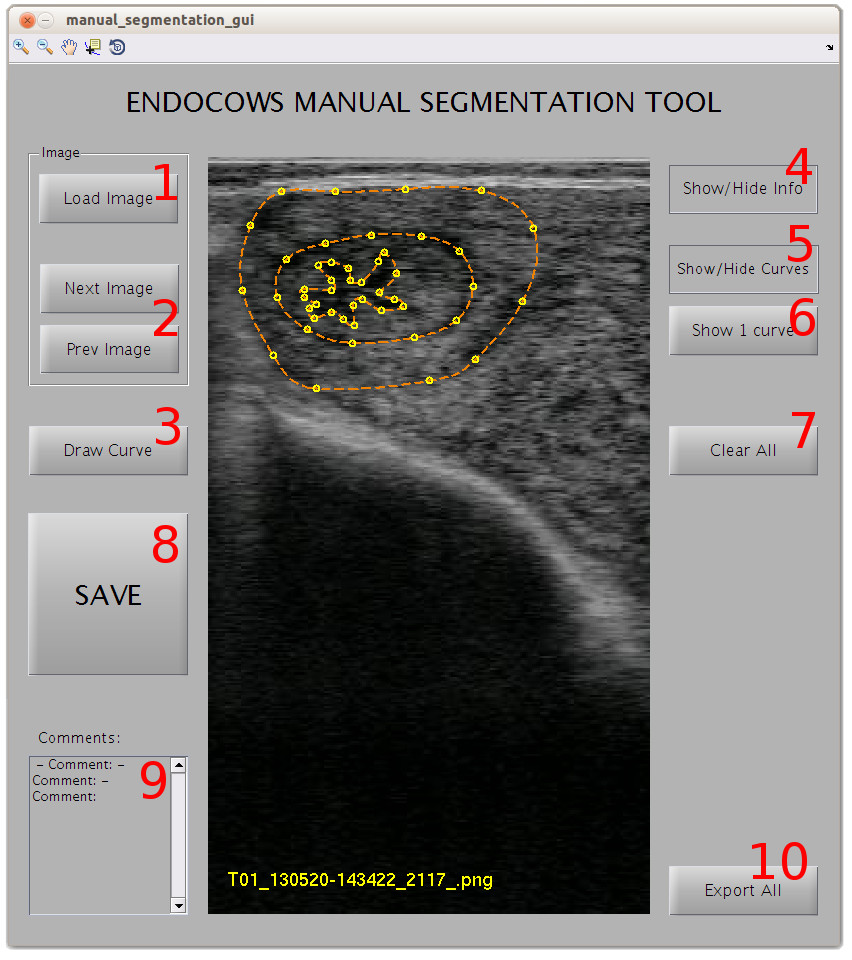
\includegraphics[width=1\textwidth]{interfaz.jpg}
	\end{center}
	\caption{User Interface}
	\label{fig:interfaz}
\end{figure}


\section{User Interface}

\begin{enumerate}
	\item \textbf{Load Image}: This button is pressed only for load the first image to segment. After that, \emph{Next Image} and \emph{Prev Image} buttons will be pressed to segment other images. After pressing \emph{Load Image} a pop-up dialog will appear in order the user can navigate to the folder that contains the images and select one to segment.
	\item \textbf{Next and Prev Image}: This buttons are used to navigate between images in the same folder (the one selected in the step before, with \emph{Load Image} button).
	\item \textbf{Draw Curve}: Button for drawing a closed curve to segment Miometrio, Endometrio and Lumen (if necessary). After pressing this button a crosshair will appear over the mouse cursor. Each \emph{left click} will add a control point for the curve. 
	%The last control point of the curve needs to be done by clicking the right button of the mouse. 
	%It is important to highlight that the curve is finalized if and only if the user makes a right click over the image
	\emph{To finalize the curve a right click over the image is needed.}
	\item \textbf{Show/Hide Info}: As can be noticed in figure \ref{fig:interfaz}, a legend is printed on the lower part of the image, showing the name of the image file. The toggle button \emph{Show/Hide Info} is used to show or hide this legend. Each time the button is pressed, alternates between showing or hiding the legend.
	\item \textbf{Show/Hide Curves}: As the previous one, this is also a toggle button. Each time this button is pressed, it alternates between showing or not saved curves. By default, this button is pressed, which means that when a new image is loaded (by \emph{Load Image}, \emph{Next Image} or \emph{Prev Image}), the program looks for all saved curves in current path and shows them. If the button is turned off, the program will no longer show the saved curves.
	\item \textbf{Show 1 curve}: This button shows a pop-up window so as the user can select which curve to show. By default the pop-up window shows only saved curves for the current image, but has the options for showing all saved curves for the current patient, or all the saved curves in the current path.
	\item \textbf{Clear all}: This button clears all curves shown. It will not erase the saved curves file.
	\item \textbf{SAVE}: By clicking this button all curves drew in the current image will be saved to a \emph{.mat} file in the current directory. \textbf{Do not forget to save curves!}
	\item \textbf{Comments}: This field is meant to be used for the user to write down some comments about the image, the curves or the diagnostic. If Endometritis is found, \textbf{do not forget to write it down here!}
	\item \textbf{Export All}: By clicking this button, a folder named \textbf{logs} will be created (if it does not exist) inside the images folder and will save a \emph{.tar} file containing all saved curves for all images in the current folder. It makes easier to share results with us.
\end{enumerate}


\section{Instructions for usage}

\begin{enumerate}
	\item First of all we need to uncompress the \emph{.zip} with the code in certain folder. Let me call it \emph{src\_path}.
	\item Localize the images folder and let me call it \emph{images\_path}.
	\item Open up \emph{MatLab}
	\item It will probably open in a working directory, different from both \emph{src\_path} and \emph{images\_path}, so the first thing we need to do is navigate to \emph{src\_path}. How do we do that? 
	\begin{itemize}
		\item In the upper part of Matlab main window there is a \emph{Current Folder Toolbar}. We need to use it to navigate to our \emph{scr\_path}. The are various ways to get this done. The easiest way is to click the ``>>'' symbol shown in said toolbar repeatedly up to we arrive to the \emph{src\_path}. The other way is to click the folder icon shown in said toolbar and navigate to the \emph{src\_path}.
	\end{itemize}
	\item Place the cursor in the Matlab main windows by clicking anywhere inside that window
	\item Type \emph{manual\_segmentation\_gui} and press Enter
	\item The main interface will appear, like the one shown in figure \ref{fig:interfaz}.
	\item Do not forget to save curves!
\end{enumerate}



\end{document}